\documentclass[a4paper,12pt]{article}
\usepackage{graphicx}
\usepackage{titlesec}
\usepackage[utf8]{inputenc}
\usepackage{xcolor}
\usepackage{fancyhdr}
\usepackage{lipsum}
\usepackage{caption}
\usepackage{floatrow}
\usepackage{lmodern}

\renewcommand{\headrulewidth}{0pt}
\fancyhead[C]{}
\fancyhead[C]{
	
\includegraphics[width=4cm]{metu}
}
\pagestyle{plain}

%opening
\title{Middle East Technical University\\Department of Physics\\\textbf{PHYS307 Applied Modern Physics}}
\author{Oğuzhan ÖZCAN\\}
\date{}
\clearpage
\thispagestyle{empty}
\providecommand{\groupmember}[1]{\textbf{Group Members:} }
\providecommand{\expdate}[1]{\textbf{Experiment Date:} }
\providecommand{\repdate}[1]{\textbf{Report Submit Date:} }
\providecommand{\expname}[1]{\textbf{Exp. MP-HE The Hall Effect} }


\usepackage[a4paper,%
left=0.5in,right=0.5in,top=0.5in,bottom=0.8in,%
footskip=.25in]{geometry}
%\topmargin -4.5cm
%\oddsidemargin 0.2cm
%\textwidth 16cm %
%\textheight 21cm%
%\footskip 1.0cm%




\begin{document}
\pagenumbering{gobble}
\maketitle

\thispagestyle{fancy}

%%%%%%%%%%%%%%%%%%%%%%%%%%%%%%%%%%%%%%%%%%%%%%%%%%%%%
\noindent\rule{18.4cm}{0.8pt}
\begin{center}
	\expname{arg1}{}
\end{center}

\expdate{November 6, 2015}{December 4, 2015}\\
\repdate{arg1}{December 11, 2015}\\
\noindent\rule{18.4cm}{0.8pt}\\\\
%%%%%%%%%%%%%%%%%%%%%%%%%%%%%%%%%%%%%%%%%%%%%%%%%%%%%
\begin{table}[h!]
\begin{center}
	\begin{tabular}{|c|c|}
	\hline Sample Current - $I_{p}$ (mA) & Hall Voltage - $U_{H}$ (mV) \\ 
	\hline -30 & -39.6 \\ 
	\hline -25 & -32.1 \\ 
	\hline -20 & -23.7 \\ 
	\hline -15 & -15.2 \\ 
	\hline -10 & -8.3 \\ 
	\hline -5 & 0.7 \\ 
	\hline 0 & 7.7 \\ 
	\hline 5 & 15.7 \\ 
	\hline 10 & 24.8 \\ 
	\hline 15 & 32.4 \\ 
	\hline 20 & 39.7 \\ 
	\hline 25 & 48 \\ 
	\hline 30 & 55.6 \\ 
	\hline 
\end{tabular}
\caption{Hall Voltage as a function of Sample Current}
\end{center} 
\end{table}
\begin{center}
\textbf{Slope m=1.6 mV/mA}
\end{center}
\textbullet 	The charge carrier concentration from ($U_{H}$ versus $I_{p}$) =$8.1 \times 10^{20}$ m$^{-3}$\\
\textbullet 	Type of Germanium semiconductor used = \textit{p-type}
\newpage
\begin{table}[h!]
	\begin{center}
		\begin{tabular}{|c|c|c|}
	\hline Flux Denstiy - $B$ (mT) & Hall Voltage - $U_{H}$ (mV) & Sample Voltage - $U_{p}$ (mV) \\ 
	\hline 0 & -1.3 & 1.80 \\ 
	\hline 15 & 2.5 & 1.80 \\ 
	\hline 30 & 6.0 & 1.80 \\ 
	\hline 45 & 10.2 & 1.81 \\ 
	\hline 60 & 13.4 & 1.81 \\ 
	\hline 75 & 17.0 & 1.81 \\ 
	\hline 90 & 20.6 & 1.81 \\ 
	\hline 105 & 24.3 & 1.81 \\ 
	\hline 120 & 27.4 & 1.81 \\ 
	\hline 135 & 30.6 & 1.81 \\ 
	\hline 150 & 34.7 & 1.82 \\ 
	\hline 165 & 37.9 & 1.82 \\ 
	\hline 180 & 41.5 & 1.83 \\ 
	\hline 195 & 44.3 & 1.83 \\ 
	\hline 210 & 48.0 & 1.83 \\ 
	\hline 225 & 50.7 & 1.83 \\ 
	\hline 240 & 54.0 & 1.84 \\ 
	\hline 255 & 57.3 & 1.84 \\ 
	\hline 270 & 60.3 & 1.84 \\ 
	\hline 285 & 63.4 & 1.85 \\ 
	\hline 300 & 66.1 & 1.85 \\ 
	\hline 
\end{tabular} 
\caption{Hall Voltage and the Sample Voltage as a function of Flux Density}
	\end{center}
\end{table}
\begin{center}
	\textbf{Slope m=0.2 mV/mT}
\end{center}
\begin{figure}[h!]
\centering
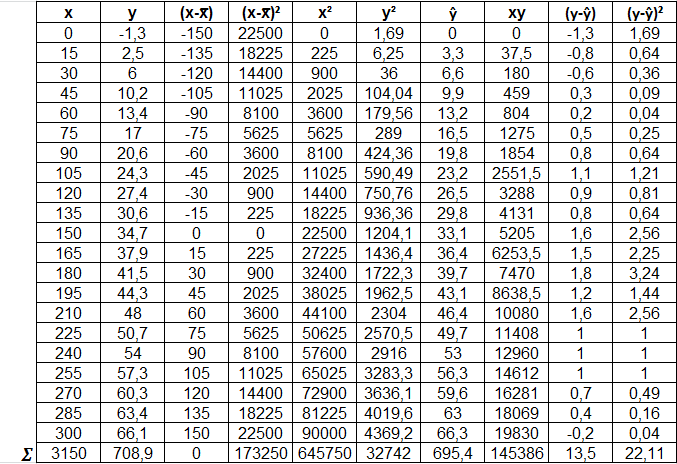
\includegraphics[width=0.8\linewidth, height=0.28\textheight]{Fig}
\caption{Terms calculate the slope and error in the slope of Hall Voltage versus Field Strength ($x=B$, $y=U_{H}$)}
\label{fig:Fig}
\end{figure}
\newpage
Sum of some important values:\\
$\sum x$ = 3150\\
$\sum y$ = 708.9\\
$\sum x^{2}$ = 645750\\
$\sum y^{2}$ = 32742\\
$\sum xy$ = 145386\\
$\sum (y-\hat{y})^{2}$ = 22.11\\
$\sum (x-\bar{x})^{2}$ = 173250\\\\
e. Find slope by the use of following formula
\begin{equation}
m=\frac{145386 - \frac{\sum x \sum y}{n}}{\sum x^{2} - \frac{(\sum x )^{2}}{n}}
\end{equation}
\begin{equation}
m=\frac{\sum xy - \frac{3150 \times 708.9}{21}}{645750 - \frac{(3150)^{2}}{21}}
\end{equation}
\begin{equation}
m=\frac{39051}{173250}
\end{equation}
\begin{center}
	\framebox[100pt]{m=0.225}
\end{center}
Then find the charge carrier concentration $n$ by the use of following formula
\begin{equation}
n=\frac{I}{mqd}
\end{equation}
where I=0.03 A, d=0.001 m and q=$1.602\times10^{-19}$
\begin{equation}
n=\frac{0.03}{0.001 \cdot 1.602\times 10^{-19} \cdot 0.225}
\end{equation}
\begin{center}
\framebox[100pt]{$n=8.32\times10^{20}$}
\end{center}
f. Find $\Delta m$ (standard error in the original slope) by the use of following formula
\begin{equation}
\Delta m = \sqrt{\frac{\frac{1}{n-2}\sum (y-\hat{y})^{2}}{\sum (x-\bar{x})^{2}}}
\end{equation}
\begin{equation}
\Delta m = \sqrt{\frac{\frac{1}{19}22.11}{173250}}
\end{equation}
\begin{center}
	\framebox[100pt]{$\Delta m =0.00259$}
\end{center}
The standard error in carrier concentration is
\begin{equation}
\Delta n = \frac{n^{2}}{K}\times\Delta m
\end{equation}
\newpage
where $K= \frac{I}{qd}$ which is equal to $1.87\times10^{20}$ in this case

\begin{equation}
\Delta n = \frac{(8.32\times 10^{20})^{2}}{1.87\times 10^{20}}\times 0.00259
\end{equation}
\begin{center}
	\framebox[100pt]{$\Delta n =9.58\times 10^{18}$}
\end{center}
So,
\begin{center}
	\framebox[200pt]{n = $8.32\times 10^{20} \pm 9.58\times 10^{18}$ m$^{-3}$}
\end{center}
\textbf{1. Explain how did you find out the type of semiconductor.}\\\\
As we can see in Table 1, slope is positive (m=1.6). Since slope is positive, we can say that this is a p-type semiconductor.\\\\
\textbf{2. a) A piece of semiconductor with the Hall coefficient $6.3\times 10^{-4}$ m$^{3}$C$^{-1}$ is used to make a Hall probe. A current of 2.0 mA is passed along the 10 mm length of the probe. The width of the face to be placed perpendicular to the uniform magnetic field measures 5 mm and the thickness is 1 mm. Estimate the Hall potential difference which would be obtained when B is 0.3 T.}\\\\
As we know, Hall coefficient $R_{H}$ is equal to $\frac{1}{nq}$. Hall potential $V_{H}$
\begin{equation}
V_{H}=\frac{1}{nq}\frac{IB}{d}
\end{equation}
Therefore Hall potential $V_{H}$ will be
\begin{equation}
V_{H}=6.3\times 10^{-4} \frac{0.3 \cdot 2.0\times 10^{-3}}{1.0 \times 10^{-3}}
\end{equation}
\begin{center}
	\framebox[150pt]{$V_{H}=3.78 \times 10^{-4}$ V}
\end{center}
\textbf{b) Find the speed of the charge carriers in the semiconductor given above.}
\begin{equation}
v=\frac{1}{nq}\frac{I}{A}
\end{equation}
where $A$ is cross-sectional area of semiconductor
\begin{equation}
v=6.3 \times 10^{-4} \frac{2.0\times 10^{-3}}{5\times 10^{-5}}
\end{equation}
\begin{center}
	\framebox[150pt]{$v$= 0.0252 m/s}
\end{center}
\newpage
\textbf{3. Explain how and why does the sample voltage change with magnetic field strength ($U_{P}-B$).}\\\\
The resistance of the sample increases with the increase of magnetic. Ohm's Law stated the relation between resistance and voltage clearly as
\begin{equation}
V=IR
\end{equation}
Since resistance $R$ increase, voltage $V$ also increases. This phenomenon is known as magnetoresistance which is due to the fact that the drift velocity of all carriers is not the same. \\\\
\textbf{4. Explain how and why does the Hall voltage change with magnetic field strength ($V_{H}-B$).}\\\\
The Hall Voltage is a linear function of the applied magnetic field. This relation can be expressed mathematically as
\begin{equation}
V_{H}=-wvB
\end{equation}
where $B$ is the magnetic field strength. When a magnetic field is applied to across the semiconductor or any material which is perpendicular to the current path, Lorentz forces cause a slight shift in the current path because they do in traditional Hall effect. This is causes a voltage differential. As we mentioned above, Hall voltage is proportional to the magnetic field and also related with the drift velocity. In a known magnetic field, drift velocity can be calculated by using Hall voltage.\\\\
\textbf{Discussion and Conclusion}\\\\
In this experiment we carried out a crucial topic in physics which is Hall Effect. Hall effect is widely using in some like Solid State Physics. When we put a conductor in a magnetic field then a voltage difference can be observed across the conductor. By using Hall Effect, today, we can detect the type of a semiconductor wheter is a p-type or n-type. While talking about Hall effect, we should explain the Hall Coefficient $R_{H}$ which is equal to $1/nq$. In this experiment we used a Germanium semiconductor which is the intrinsic semiconductor. We applied different voltage and current to our semiconductor and we observed that each one can effect the magnetic field stregth. Obviously, changing in magnetic field stregth also effect voltage and current. There is one issue that we did not studied in the experiment that is the behaviour of voltage and current in different temperature. As we state in Table 2, slope is 0.2 mV/mT. After calculations whose are stated in Figure 1 we can see that slope m is equal to 0.225 mV/mT. In Figure 3 and 4 we stated theoretical and experimental values for Hall Voltage. Since there is a small difference between them we can calculate a percentage error as follows 
\begin{equation}
Percentage Error=\frac{|0.22-0.23|}{0.22}\times 100\%=4.5\%
\end{equation}
To sum up, we can say that this experiment was successful and data that we took in experiment is acceptable.


\newpage
\textbf{{\LARGE Plots}}
\begin{figure}[h!]
\centering
\includegraphics[scale = 0.60]{"Sample Current plot"}
\caption{Hall Voltage versus Sample Current}
\label{fig:SampleCurrentplot}
\end{figure}

\begin{figure}[!h]
	\begin{floatrow}
		\ffigbox{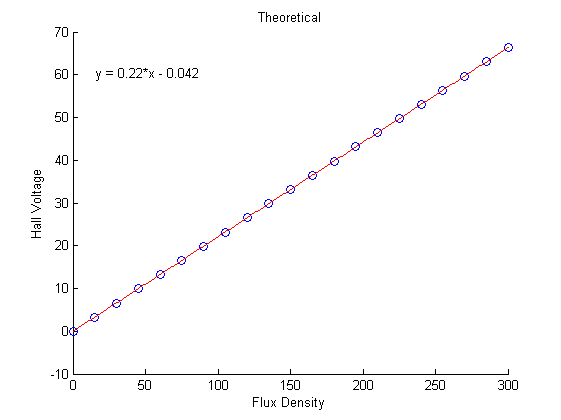
\includegraphics[scale = 0.60]{theo}}{\caption{Hall Voltage versus Flux Density Theoretical Value}\label{fig:theo}}
		\ffigbox{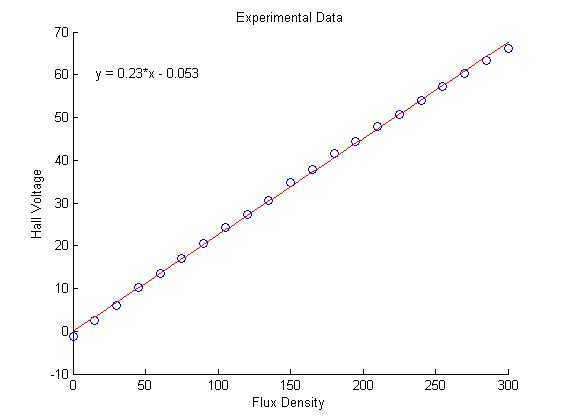
\includegraphics[scale = 0.60]{exp}}{\caption{Hall Voltage versus Flux Density Experimental Value}\label{fig:exp}}
	\end{floatrow}
\end{figure}




























































































































\end{document}
